\subsection{Definicje}
Definicje zostały zaczerpnięte z literatury, z pozycji \cite{Wloch2008}, \cite{Wilson2012} oraz \cite{Wojciechwoski2013}.

\newcommand{\graphDefinitionIndex}{1}
\newcommand{\incrementGraphDefinitionIndex} {
    \pgfmathtruncatemacro{\graphDefinitionIndex}{\graphDefinitionIndex + 1}
}

\noindent
\textbf{Definicja \graphDefinitionIndex.}
\incrementGraphDefinitionIndex
Grafem nieskierowanym, skończonym $G$ nazywamy parę $(V,E)$, gdzie $V = V(G)$ jest zbiorem skończonym, niepustym,
natomiast $E = E(G)$ jest rodziną mogących się powtarzać dwuelementowych podzbiorów niekoniecznie różnych elementów ze zbioru $V$.
Zbiór $V(G)$ nazywamy zbiorem wierzchołków, a elementy tego zbioru nazywamy wierzchołkami i oznaczamy symbolami:
$x$, $y$, $x_i$, $y_i$, $1$, $2$, ... Zbiór $E(G)$ nazywamy zbiorem krawędzi grafu $G$.
Mówimy, że krawędź $\{v, w\}$ łączy wierzchołki $v$ i $w$, i na ogół oznaczamy ją krócej symbolem $vw$.
W wielu zagadnieniach nazwy wierzchołków są nieistotne, więc je pomijamy i mówimy wtedy, że graf jest nieoznakowany.

\noindent
\textbf{Definicja \graphDefinitionIndex.}
\incrementGraphDefinitionIndex
Jeżeli w grafie $G$ istnieją co najmniej dwie krawędzie $xy$, to krawędź tę nazywamy krawędzią wielokrotną.

\noindent
\textbf{Definicja \graphDefinitionIndex.}
\incrementGraphDefinitionIndex
Krawędź $xy$ w grafie $G$ nazywamy pętlą.

\noindent
\textbf{Definicja \graphDefinitionIndex.}
\incrementGraphDefinitionIndex
Graf mający krawędzie wielokrotne nazywamy multigrafem.

\noindent
\textbf{Definicja \graphDefinitionIndex.}
\incrementGraphDefinitionIndex
Graf, który nie ma krawędzi wielokrotnych i pętli, nazywamy grafem prostym.

\noindent
\textbf{Definicja \graphDefinitionIndex.}
\incrementGraphDefinitionIndex
Graf zawierający pętle nazywamy pseudografem.

\noindent
\textbf{Definicja \graphDefinitionIndex.}
\incrementGraphDefinitionIndex
% Wierchołek izolowany ---------------------------------- to do

\noindent
\textbf{Definicja \graphDefinitionIndex.}
\incrementGraphDefinitionIndex
Graf $G$ taki, że $E(G) = \emptyset$, nazywamy grafem bezkrawędziowym. Jeżeli $|V(G)| = n$, to graf bezkrawędziowy oznaczony symbolem $N_n$.
Każdy wierchołek grafu bezkrawędziowego jest wierchołkiem izolowanym.

\noindent
\textbf{Definicja \graphDefinitionIndex.}
\incrementGraphDefinitionIndex
% Wierchołki sąsiednie ---------------------------------- to do

\noindent
\textbf{Definicja \graphDefinitionIndex.}
\incrementGraphDefinitionIndex
Graf prosty $G$ taki, że każde dwa wierzchołki są sąsiednie, nazywamy grafem pełnym.
Jeżeli $|V(G)| = n$, to graf pełny oznaczamy $K_n$.

\noindent
\textbf{Definicja \graphDefinitionIndex.}
\incrementGraphDefinitionIndex
Graf G, którego zbiór wierchołków można podzielić na dwa rozłączne, niepuste podzbiory $V_1$ i $V_2$ tak,
że jeżeli $xy \in E(G)$, to $x \in V_1 \vee y \in V_2$ nazywamy grafem dwudzielnym.
% Sprawdzić znak LUB (usunąć?) ---------------------------------- to do

\noindent
\textbf{Definicja \graphDefinitionIndex.}
\incrementGraphDefinitionIndex
Drogą w grafie jest skończony ciąg naprzemiennie występujących wierzchołków i krawędzi, rozpoczynający się
i kończący wierzchołkami, taki, że każde dwie kolejno po sobie następujące krawędzie mają wspólny wierzchołek.

\noindent
\textbf{Definicja \graphDefinitionIndex.}
\incrementGraphDefinitionIndex
% Graf skierowany ---------------------------------- to do

\begin{figure}[ht]
	\centering
	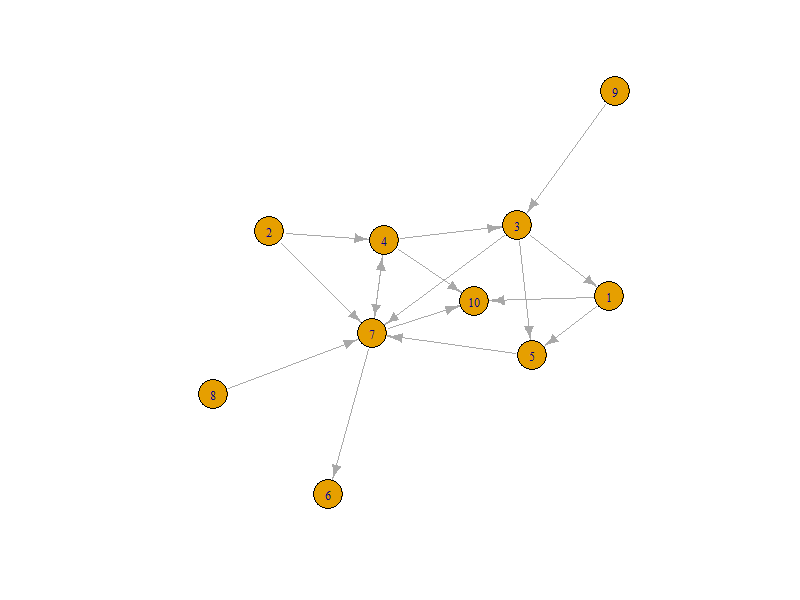
\includegraphics[height=8cm]{partials/images/graph_directed.png}
	\caption{Przykład grafu skierowanego}
	\label{Fig:graphs-undirected-1}
\end{figure}
\FloatBarrier

\begin{figure}[ht]
	\centering
	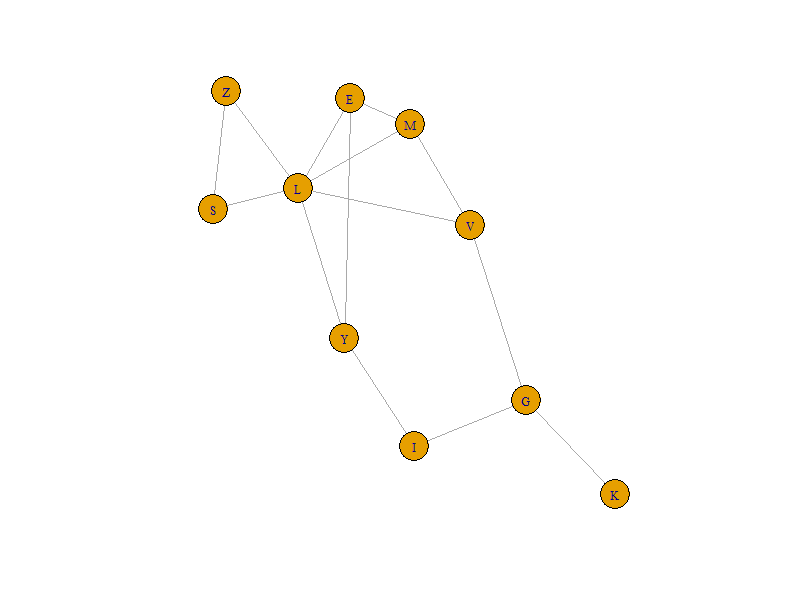
\includegraphics[height=8cm]{partials/images/graph_undirected.png}
	\caption{Przykład grafu nieskierowanego}
	\label{Fig:graphs-directed-1}
\end{figure}
\FloatBarrier